\documentclass{article}
\usepackage[utf8]{inputenc}
\usepackage{amsmath}
\usepackage{tcolorbox}
\usepackage{amssymb}
\usepackage{amsthm}
\usepackage{proof}
\usepackage{float}
\theoremstyle{definition}


\usepackage[
top    = 2.50cm,
bottom = 2.50cm,
left   = 2.75cm,
right  = 2.75cm]{geometry}
\usepackage{fancyhdr}
\pagestyle{fancy}
\lhead{Advanced computation}
\rhead{EPFL/Alp Ozen}
\newcommand{\floor}[1]{\lfloor #1 \rfloor}

\title{Advanced Computation 1 - CS 101}
\author{Alp Ozen}
\date{\vspace{-5ex}}
\newtheorem{theorem}{Theorem}[section]
\newtheorem{example}{Example}
\newtheorem{remark}{Remark}
\newtheorem{definition}{Definition}
\numberwithin{equation}{subsection}
\numberwithin{remark}{subsection}
\newtheorem{question}{Question \textit{???}}
\begin{document}

\maketitle
\section{Propositional logic and notions of sets(Week 1 - Week 4)}
\subsection{Propositions}
A proposition is a declarative sentence that is either true or false. 
\begin{tcolorbox}
How much does it cost? \textbf{is not a proposition}
\\
I like red \textbf{is a proposition}
\end{tcolorbox}

To make life easier, we represent propositional statements through letters such as $p$. 
\\

The conditional statement $p\implies q$ appears very often. Thus, we have the \textit{converse,contrapositive and inverse} which are:
\\
\textbf{converse}: $q \implies p$
\\
\textbf{contrapositive}: $ \neg q \implies \neg p $
\\
\textbf{inverse}: $ \neg p \implies \neg q$
\\

We note that a conditional is logically equivalent to its contrapositive. 

\begin{tcolorbox}
\centering
\begin{array}{cccccc}
 p & q & p $\implies$ q & \neg q & \neg p & \neg q $\implies$ \neg p \\
 \hline
t & t & t & f & f & t\\
t & f & f & t & f & f\\
f & t & t & f & t & t\\
f & f & t & t & t & t
\end{array}
\end{tcolorbox}

\subsection{Precedence of logical operators}

\begin{figure}[h]
    \centering
    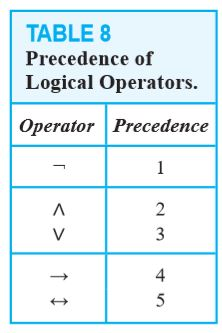
\includegraphics{figures/precedence}
\end{figure}

\subsection{Fuzzy logic}

In fuzzy logic, truth values are between 0 and 1. So if the statement "I like riding a bike" has a value of 0.8, it's negation has 1 minus this value, in this case -0.2. 

\subsection{Applications of logic}
\subsubsection{Logic gates}
Here are the basic logic circuits from which more complex circuits are made: 

\begin{figure}[h]
    \centering
    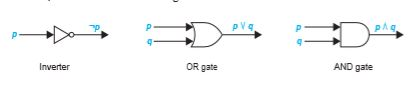
\includegraphics[scale= 1]{epflSemesterOne/advancedComputation/figures/logicgates.JPG}
    \caption{Logic gates}
    \label{fig:my_label}
\end{figure}

Note that the OR and AND gates accept only and only 2 inputs and output one. This input may be as compounded as possible but not exceed 'two chunks'. Thus, when given a complex logical output and reverse engineering, we identify the outer most outer operation, branch it into two or one(if it is simply a negation) and so on. 

\subsubsection{More on propositions}

\begin{tcolorbox}
\begin{itemize}
    \item \textbf{Tautology} is a compound proposition that is always true regardless of the truth value of its variables
    \item \textbf{Contradiction} is a compound proposition that is always false regardless of the truth value of its variables 
    \item \textbf{Contingency} compound statement that is neither tautology nor contradiction
    
    \begin{example}
    \\
    $p \land \neg p$ is a contradiction
    \\
    $p \lor \neg p$ is a tautology
    \end{example}
\end{itemize}
\end{tcolorbox}

Here are some examples of logical calculus:
\\
Show that $\neg(p \lor (\neg p \land q )) \equiveq \neg p \land \neg q$
\begin{align*}
    \neg(p\lor\neg p \land p \lor q)\\
    \neg(T \land p \lor q)\\
    \neg(p \lor q)\\
    \neg p \land \neg q
\end{align*}

\subsubsection{Satisfiability}

A compound proposition is \textbf{satisfiable} if a truth assignment can be made to its variables that make it true making it either a tautology or a contingency. It is \textbf{unsatisfiable} if the negation of the compound statement is a contradiction. 

\subsection{Logical calculus and useful equivalences}

\begin{definition}
If $A \iff B$ is a tautology, then A is logically equivalent to B. 
\end{definition}
\\

Here are some useful logical equivalences(omitting most obvious ones):

\begin{align*}
    p \implies q \equiv \neg p \lor q \equiv \neg(\neg q \lor p) \equiv \neg(q \implies p) \equiv \neg q \implies \neg p \\
    p \lor ( q \land r) \equiv (p \lor q) \land (p \lor r) \\
    \land \ \text{distributes over} \lor \text{and vice versa}\\
    p \lor \neg p \equiv T\\
    p \land \neg p \equiv F\\
    P \land T \equiv p\\
    p \lor F \equiv p
    \ \text{both $\land$ and $\lor$ are associative}
\end{align*}

For more see this figure:

\begin{figure}[h]
    \centering
    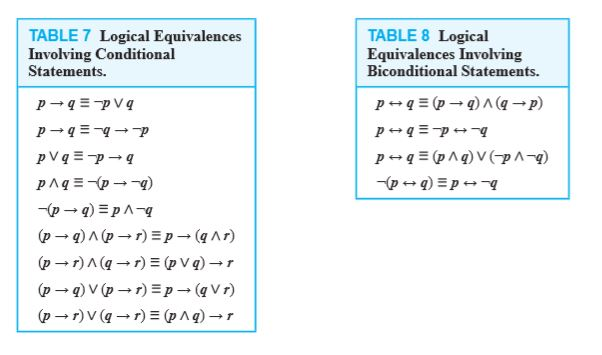
\includegraphics[scale = 0.7]{epflSemesterOne/advancedComputation/figures/logic.JPG}
    \caption{Logic, yey!}
    \label{fig:my_label}
\end{figure}

\begin{definition}
A \textbf{rule of inference} is based on the tautology $p \land (p \implies q) \implies q$. That is, whenever we are given that both $p$ and $p \implies q$ is true, we infer that q must be true. That is :
\\

\infer{q}{p & (p \implies q)}
\end{definition}

Another important fact of logic is that we may boil down all of $\lor, \oplus, \implies, \iff$ to simply propositions involving$\neg, \land$: 

\begin{align*}
    p \lor q \equiv \neg \neg (p \lor q) \equiv \neg(\neg p \land \neg q)\\
    p \oplus q \equiv \neg(p \land q) \land (p \lor q)\\
    p \implies q \equiv \neg p \lor q \equiv \neg (p \land \neg q)\\
    p \iff q \equiv \neg(\neg(p\land q) \land (\neg (\neg p \land \neg q))
\end{align*}


\begin{question}
Given propositional variables and truth values of the single variables for which the compound proposition takes a value, is there a way of deducing a compound proposition? 
\end{question}
\newpage
\subsection{Lec.03 notes}

The \textbf{contrapositive} is the following statement:
\begin{align*}
    p \implies q \equiv \neg p \lor q\\
    \equiv q \lor \neg p\\
    \equiv \neg q \implies \neg p\\
    \therefore p \implies q \equiv \neg q \implies \neg p
\end{align*}
\\
Some useful logical equivalences involving implication:

\begin{align*}
    (p \implies q) \land (p \implies r) \equiv (\neg p \lor q) \land (\neg p \lor r)\\
    \equiv \neg p \lor (q \land r) \equiv p \implies (q \land r)
\end{align*}
And here's a more trivial one: 
\begin{align*}
    (p \implies q) \lor (p \implies r) \equiv (\neg p \lor q) \lor (\neg p \lor r)\\
    \equiv \neg p \lor \neg p \lor q \lor r \equiv \neg p \lor (q \lor r)\\
    \equiv p \implies (q \lor r)
\end{align*}
And slightly more complicated involving De Morgan:
\begin{align*}
    (p \implies r) \land (q \implies r) \equiv (\neg p \lor r) \land (\neg q \lor r)\\
    \equiv \neg r \lor (\neg p \land \neg q) \equiv \neg r \lor (\neg(p \lor q)\\
    \equiv (p \lor q) \implies r 
\end{align*}

We must also add some comments on base b systems of numbers and a general algorithm for conversion. Let's take an example in base 5. Suppose we want to convert $60_{10}$ to its base 5 representation. Well the largest power of 5 less than or equal to 60 is 25 and thus we know that 60 can be \textbf{uniquely} represented as a linear combination of the powers of 5 less than or equal to it. In fact, using powers of 5 less than or equal to 60, we may represent all numbers up to $5^k - 1$ as $4\cdot5^{k-1} + \ldots + 4\cdot5^{0}$. Thus, to represent some $l$ in base $b$ the algorithm is to find the largest power of $b^k < l$, perform $\floor{\frac{l}{b^k}}$ then repeat step 1 and proceed as $l - b^k\cdot\floor{\frac{l}{b^k}}$ and repeat until $l - b^i\cdot\floor{\frac{l}{b^i}} = 0$
 
\subsection{Lec.04 notes}
\subsubsection{More on CMOS}
This was a lecture with a steep curve and here is a summary. First of all, we first revisit some of the concepts of the pmos and nmos resistors. A very important convention is that pmos must never be used for pull-down(connected to GND) and nmos never used for pullup(connected to VDD). 

\begin{figure}[h]
    \centering
    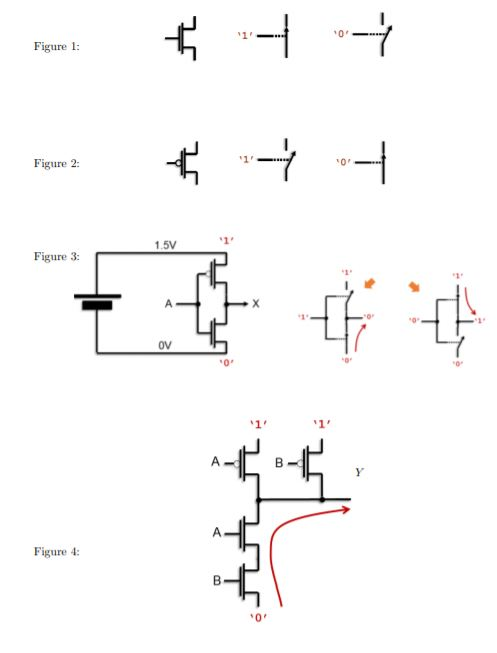
\includegraphics[scale=0.7]{epflSemesterOne/advancedComputation/figures/cmos.JPG}
    \caption{Caption}
    \label{Nmos,Pmos,Inverter,Nand}
\end{figure}

\begin{tcolorbox}
Some principles of cmos gates: 
\begin{itemize}
    \item Pmos goes to top, nmos to bottom.
    \item Never connect high voltage to low voltage to prevent a short circuit. 
    \item Any circuit may be realized as a combination of the NAND and NOR ciruit. 
    \item Each pmos must connect to an nmos. 
\end{itemize}
\end{tcolorbox}
\\
The most challenging part of CMOS circuits is the circuit analysis itself. Consider this example to see a method of circuit analysis: 


\begin{figure}[h!]
    \centering
    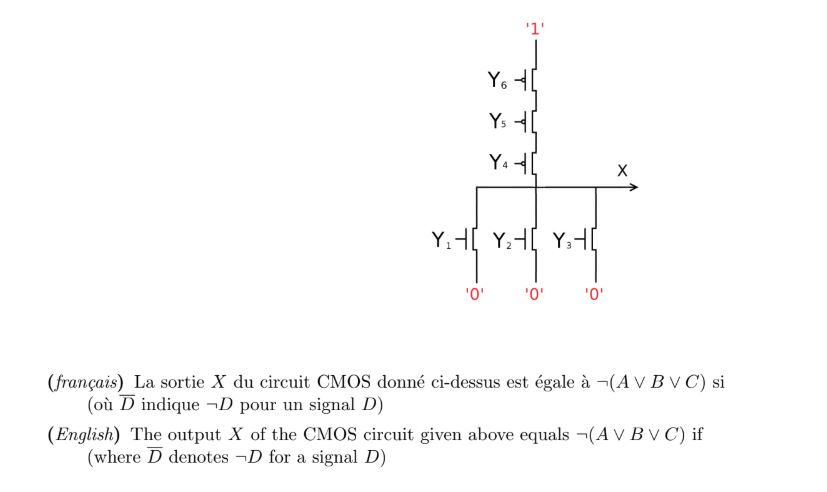
\includegraphics[scale = 0.6]{epflSemesterOne/advancedComputation/figures/cmosq.JPG}
    \caption{exam question}
    \label{exam question}
\end{figure}

\FloatBarrier

\begin{tcolorbox}
Now, first of all, realize that X is connected to VDD iff all of $Y_{6} \land Y_{5} \land Y_{4}$ are grounded. That is $Y_{6} \land Y_{5} \land Y_{4} = 0$. For symbolic purposes, supposing that $Y_{i} = 0 \equiv \neg Y_{i} $ we get that $X = 1 \iff \neg (Y_{4} \lor Y_{5} \lor Y_{6})$ Now given that this is a CMOS circuit, we know that the bottom part does the exact opposite of the upper part. Thus, we have that $X=0 \iff \neg(\neg (Y_{4} \lor Y_{5} \lor Y_{6})) = Y_{4} \lor Y_{5} \lor Y_{6} \equiv Y_{1} \lor Y_{2} \lor Y_{3}$. As a final step, for $\neg (A \lor B \lor C)$ to be true, we need that the output equals $\neg(A \lor B \lor C)$ and since $X=1 \iff \neg (Y_{4} \lor Y_{5} \lor Y_{6})$ we get that $Y_{1} = Y_{2} \ldots$

\end{tcolorbox}

\subsubsection{Binary addition circuit}

Given that we can construct any compound logical gate using CMOS, suppose we want to implement a binary addition calculator. Now here are all the possible cases for doing binary addition: 

\begin{figure}[h]
    \centering
    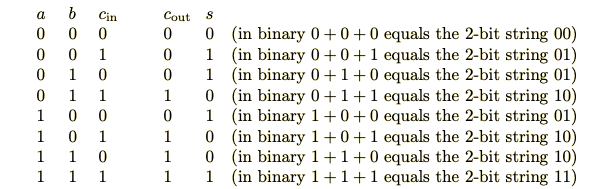
\includegraphics[scale = 0.6]{epflSemesterOne/advancedComputation/figures/binary.png}
    \caption{Addition possibilities}
    \label{fig:my_label}
\end{figure}

Now suppose we want a function $f(a,b,c_{in})$ to evaluate $s$. Well notice that $s$ is only true when the parity of $a,b,c_{in}$ is odd. That is, we may describe this outcome with the function $a \oplus b \oplus c_{in}$. Similarly, devising $g(a,b,c_{in})$ to compute $c_{out}$ we notice that $c_{out}$ evaluates to 1 iff at least two variables are true. This is equivalent to $(a\land b) \lor (a \land c_{in}) \lor (b \land c_{in})$

\subsubsection{Fast Multiplication aka. Karatsuba}
We now ponder whether there is a quick way of multiplying some $v$ and $w$. Now notice that for $v$ and $w$ in base 10, $v = aX + b$ and $w = cX + d$. Now notice that $v \cdot w = (aX+b)(cX+d)$ which in turn is:

\begin{equation*}
    v\cdot w = acX^2 + (ad + bc)X + bd
\end{equation*}

And further notice that:

\begin{equation*}
    ad + bc = (ac + bd) - (a - b)(c - d) 
\end{equation*}

to get:

\begin{equation*}
    v\cdot w = acX^2 + ((ac + bd) - (a - b)(c - d))X + bd
\end{equation*}

Now if for instance $v$ and $w$ were 2 digit numbers, we would normally perform 4 digit by digit multiplications but with this new method, we end up performing only 3 and a trivial subs traction. 
\\
As a general result, for multiplication of two k by k digit numbers, we end up performing $3^{\log_{2}k}$ multiplications and $log_{2}k$ many additions. Finally, notice that Karatsuba is a recursive algorithm. 
\subsubsection{Two's compliment}
Consider how a computer is to represent negative integers. A very smart way of doing so is \textbf{two's compliment}. That is given a binary representation, we invert all 1's with 0's and all 0's with 1's and then add 1. Note that now the 0's take the role of 1's and vice versa. The reason for adding 1 is that the most significant digit is reserved for the sign. A 1 is a negative, a 0 a positive.  
\\
\begin{remark}
Note that when multiplying two numbers with non-matching number of digits, we simply pad both numbers with 0's until both have number of digits that are a power of 2. 
\end{remark}

\subsection{Lec 05. notes}
\subsubsection{Main points}
In this lecture quantifiers and their properties were discussed along with common pitfalls. 
\\
Consider defining a proposition on some sub-domain. That is take $D = \{0,1,2\}, S = \{2\}$ Now we want to express the proposition $\forall x \in S, P(x)$ where $P(x)$ is to mean that $x$ is even in the form $\forall x Q(x)$. A major mistake made is to try and express this as $x \in S \land P(x) \equiv Q(x)$ Now clearly $\forall x Q(x) \not \equiv \forall x \in S, P(x) $ as taking $x=1$ leads to the LHS being false. So here is the correct way to do this: Let $Q(x) \equiv x\in S \rightarrow P(x)$. It is now the case that $\forall x Q(x) \equiv \forall x \in S, P(x)$. Therefore we have that:

\begin{align}
    \forall x \in S, P(x) \equiv \forall x(x\in S \rightarrow P(x))\\
    \exists x \in T P(x) \equiv \exists x( x\in T \land P(x))
\end{align}

\begin{remark}
Note that both $\exists$ and $\forall$ have precedence over any other logical operator. 
\end{remark}

We would also like to point out that whenever we have an empty domain, then both $\exists x P(x)$ and $\exists x \neg P(x)$ are both false. Similarly, $\forall x P(x)$ and $\forall x \neg P(x)$ are both true. 
\\
We now ask, how do we negate the quantifiers?

\begin{align}
    \neg(\exists x P(X)) \equiv \forall x \neg P(x)\\
    \neg(\forall x P(X)) \equiv \exists x \neg P(x) 
\end{align}
And we add the note that the same negation rules also hold for quantifiers over a sub-domain. Here is an example proof:

\begin{align*}
    \equiv \neg \forall x \in S \ P(x) \equiv \neg (\forall x \in S \rightarrow P(x))\\
    \equiv \exists x \neg(x \in S \rightarrow P(x))\\
    \equiv \exists x \neg(x \not \in S \lor P(x))\\
    \equiv \exists x (x \in S \land \neg P(x))\\
    \equiv \exits x \in S, \ \neg P(x)
\end{align*}

\subsection{Lec 06. notes}

First of all, we note that when solving CMOS problems, always check if the circuit is complementary. That is whenever the upper part is 1, lower part must be disconnected. Hence if the upper part evaluates $A\land B$, lower part must evaluate $\neg(A \land B)$

Here is a nice CMOS circuit problem from week 3:

\begin{figure}[H]
    \centering
    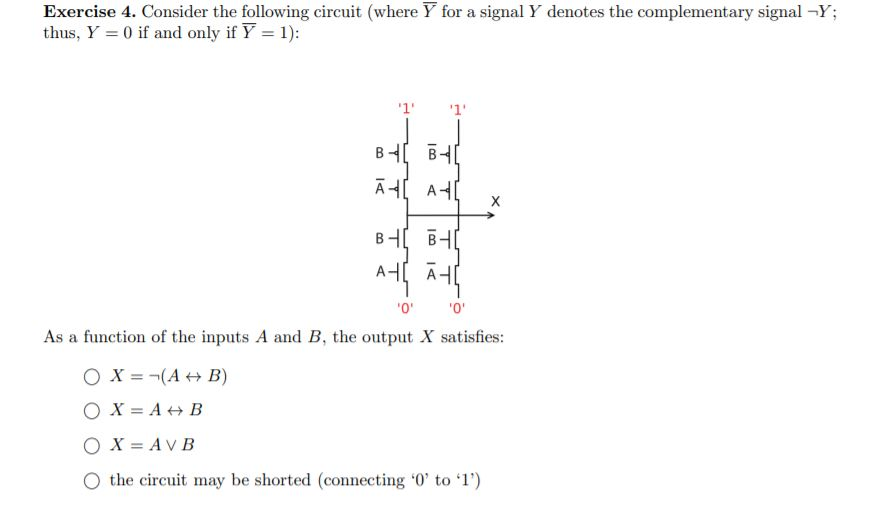
\includegraphics[scale=0.7]{epflSemesterOne/advancedComputation/figures/cmos2.JPG}
    \caption{PSET3 cmos problem}
    \label{fig:my_label}
\end{figure}

Here's how I solved it:
\\
Now notice that $X=1$ iff. $(B=0 \land \neg A = 0) \lor (\neg B = 0 \land A = 0)$ Thus we obtain:
\begin{align*}
    (\neg B \land A) \lor (B \land \neg A)\\
    \equiv \neg(B\lor \neg A) \lor \neg(\neg B \lor A)\\
    \equiv \neg(A \rightarrow B) \lor \neg(B \rightarrow A)\\
    \equiv \neg ((A \rightarrow B) \land (B \rightarrow A))\\
    \equiv \neg (A \iff B)
\end{align*}
\clearpage


And here is some more details on two's compliment:

\begin{figure}[H]
    \centering
    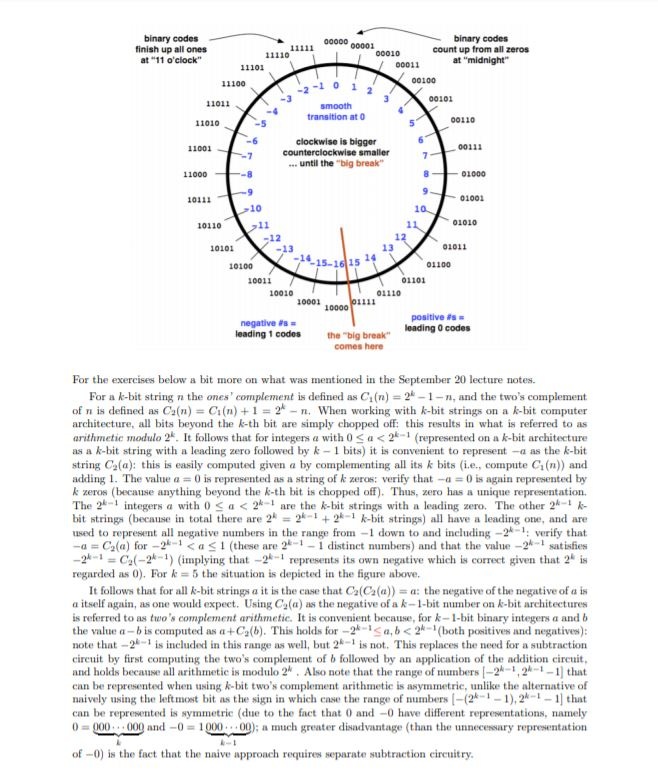
\includegraphics[scale = 1.2]{epflSemesterOne/advancedComputation/figures/twosc.JPG}
    \caption{More on two's compliment}
    \label{fig:my_label}
\end{figure}

And now let's say a little more about two's complement. That is, two's compliment simply represents the additive inverse of a number in $\bmod{2^k}$ That is, suppose we wanted some $b$ such that $a + b \equiv 0 \bmod{2^k}$, then we'd have that $b = 2^{k} - a$ Which is essentially the formula for two's complement for a given bit architecture. 


\subsection{Lec 07. notes}

We consider how to negate the $\exists!$ expression. Realize that:
$$\exists!xP(x) \equiv \exists x(P(x)\land P(y) \rightarrow (x=y))$$
And hence the negation(using our negation laws gives):
$$\neg\exists ! xP(x) \equiv P(x) \rightarrow \exists y \not = xP(y))$$
\\
And two demonstrate the importance of nesting order on quantifiers, consider this excerpt:

\begin{figure}[H]
    \centering
    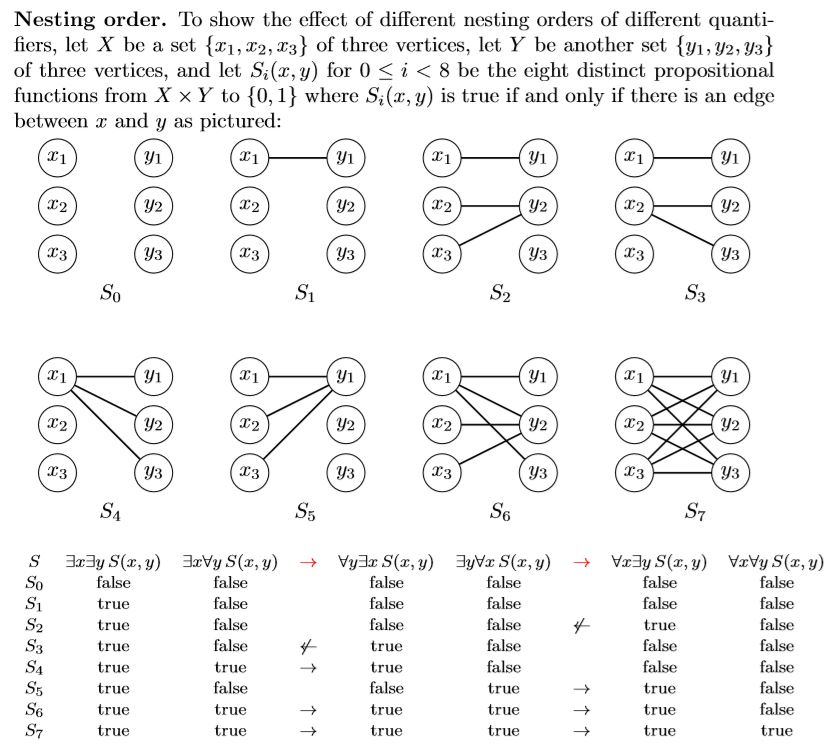
\includegraphics[scale = 0.8]{epflSemesterOne/advancedComputation/figures/nesting.JPG}
    \caption{Nesting order demo}
    \label{fig:my_label}
\end{figure}

And notice here how $\exists x \forall y S(x,y) \rightarrow \forall y \exists x S(x,y)$ This makes sense as whenever an x exists for each y, we have to have that for all y, there is an x. 
\\
\clearpage
And now we come to rules of inference for quantifiers. 

\begin{definition}(Inference laws for quantified statements)
\\
\textbf{Universal instantiation} 
\begin{equation*}
    \infer{P(c)}{\forall x P(x)}
\end{equation*}
\textbf{Universal generalization}
\begin{equation*}
        \infer{\forall x P(x)}{P(x) \text{for arbitrary x}}
\end{equation*}
And we note that the same hold respectively for the existential quantifier. 
\end{definition}

And finally we present an application of rules of inference. Suppose the following:
\\
$H(x):$ x is here
\\
$U(x):$ x likes C
\\
$L(x)$ x is a fan of D.R.(Denis Ritchie)
\\
Now we assert the following:
\\
(1) There is someone here who likes C
\\
(2) Everyone who likes C is a fan of D.R.
\\
Hence we get:
$$(1) \equiv \exists x(H(x) \land U(x))$$
$$(2) \equiv \forall x(U(x) \rightarrow L(x))$$
Now what may we infer from these?
\\
Well we know  $\exists x(H(x) \land U(x))$ hence we by instantiation we have $H(c) \land U(c)$ then $U(c),H(c)$ and since $ \forall x(U(x) \rightarrow L(x))$ to give $U(c) \rightarrow L(c), L(c)$ and finally $$H(c)\land L(c)$$
\\
And although it is not too useful to memorize their names, we include here a table of common rules of inference: 


\begin{figure}[H]
    \centering
    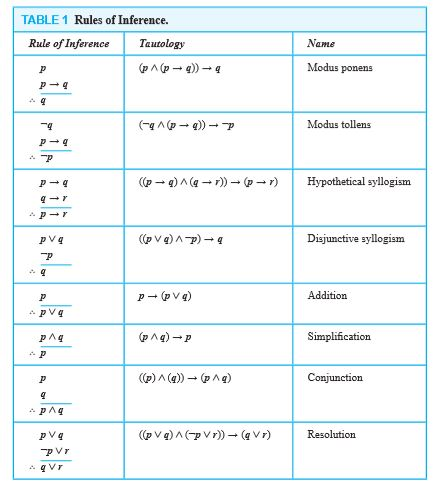
\includegraphics[scale = 0.9]{epflSemesterOne/advancedComputation/figures/inference.JPG}
    \caption{Rules of inference}
\end{figure}

\subsection{Lec 08. notes}
\subsubsection{Proof methods}
A \textbf{proof} is a valid argument establishing the truth of a statement. 
\\
We list some common proof methods and elaborate:
\\
\textbf{Direct proof:} When trying to prove a statement like $p \rightarrow q$ we consider the only case that $p \rightarrow q$ would be false and show that it can not happen. That is we take $p$ true and using our inference laws, reach that $q$ must be true as well 
\\
\textbf{Proof by contraposition:} Since $p\rightarrow q \equiv \neg q \rightarrow \neg p$ we try to show that the contrapositive holds via a direct proof. And here's a mini-example: Consider the statement \textit{if $n$ is an integer then $3n+2$ is odd.} Now suppose $3n+2$ is even to give $3n+2 = 2k, \ k\in \mathbb{N}$ Then we have that $n=\frac{2k-2}{3}$ and taking $k=2$ suffices to show $n$ is not an integer. 
\\
\textbf{Proof by contradiction:} Firstly, proof by contradiction is often confused with proof by contraposition. We use proof by contradiction to show that a statement $p$ is true. To do this, if we can show that $\neg p \rightarrow q$ is true where $q$ is always false, we have that $\neg p$ is false hence $p$ true. A common example is showing that $\sqrt{2}$ is irrational. We take the negation of $p$ that $\sqrt{2}$ is rational and derive the contradiction that whenever we try to write $\sqrt{2} = \frac{z}{k}$ with $\gcd{z}{k} = 1$ that $\gcd{z}{k} = 1 \land \gcd{z}{k} \not = 1$ Thus the falsity of $p$ implies a contradiction(false value) showing that $p$ itself must be true. 
\\
Similarly suppose we have statement $p\equiv a \rightarrow b$. We know that $\neg p \rightarrow a \land \neg b$ and get that $a\land \neg b$ is always false showing that $p$ must be true. 
\subsubsection{Graphs and planarity}
\textbf{A planar} graph is one that can be drawn without overlapping edges. Now a planar graph does not imply that for all possible drawing, overlapping edges wont exist. It simply means that a drawing could be made without overlapping edges. Now the two most important facts of graphs are:

 
 \begin{tcolorbox}[drop shadow, title=($K_{3,3}$ and $K_{5}$ are not planar),lower separated=true]
    Now notice that each connection we make partitions the plane into an inner and outer side following the \textbf{Jordan theorem}. We find out that when it comes to drawing the last vertex for $K_{3,3}$, the edge is surrounded by 4 curves making it impossible to not cross a curve. 
    \tcblower
    \centering
        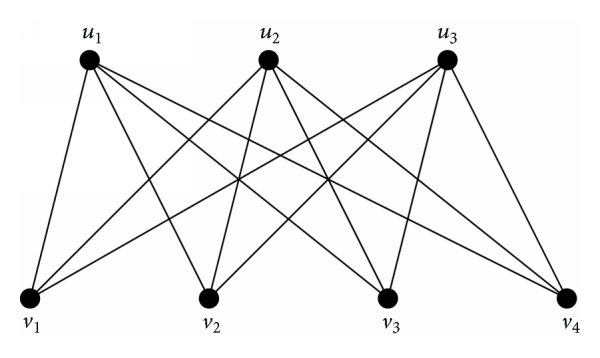
\includegraphics[scale = 1.1,valign=t]{epflSemesterOne/advancedComputation/figures/k3.png}
\end{tcolorbox}
\\
Now, \textbf{Kuratowski's theorem} states that a graph is non-planar iff it contains in one way $K_{3,3}$ or $K_{5}$
\clearpage
\subsubsection{Different surfaces}
We now consider different surfaces, those of the \textbf{Torus, Mobius strip, Klein bottle} shown respectively in the figure below. 

\begin{figure}[H]
    \centering
    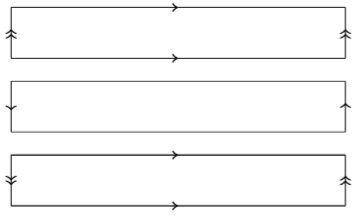
\includegraphics{epflSemesterOne/advancedComputation/figures/mobius.JPG}
    \caption{Rectangular abstraction}
\end{figure}

These surfaces are interesting because the laws of planarity no longer hold. For instance, on a mobius strip, $K_{3,3}$ is indeed planar as below. 

 \begin{tcolorbox}[drop shadow, title=($K_{3,3}$ has become planar),lower separated=true]
    \centering
        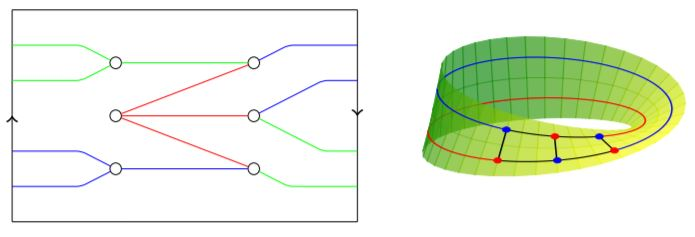
\includegraphics[scale = 0.9,valign=t]{epflSemesterOne/advancedComputation/figures/mobiusk3.JPG}
\end{tcolorbox}

\subsection{Lec 09. notes}
\subsubsection{Sequences}
We define a \textbf{sequence} as a mapping $f: \mathbb{N} \to \mathbb{R}$. Some most essential sequences are:

\begin{align*}
    \textbf{constant sequence} \ \exists c \forall i \ a_{i} = c\\
    \textbf{arithmetic sequence} \ \exists c \forall i \ a_{i+1} - a_{i}  = c\\
    \textbf{geometric sequence} \ \exists c \forall i \ \frac{a_{i+1}}{a_{i}}= c
\end{align*}
\\
More generally, the constant and arithmetic sequence are a member of the family of consecutive polynomial sequences. That is, since a polynomial is defines as:

$$\sum_{i=0}^{j} a_{i}X^{i}$$ we may have sequences of higher degree. 
\subsubsection{Summations}
Consider the summation of the first n terms of a constant sequence $a_{i} = c$. We would have $\sum_{i=1}^{n}a_{i}$ which is the same as $\sum_{i=1}^{n}c$ and taking $c=1$ we get n times 1 added which is $\sum_{i=1}^{n}c = 1$
\\
Let's now consider the summation of an arithmetic sequence by using an $nxn$ square as below: 
\begin{figure}[H]
    \centering
    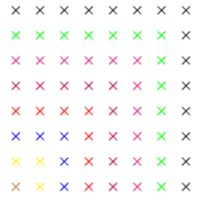
\includegraphics{epflSemesterOne/advancedComputation/figures/square.JPG}
    \caption{Summations, yey!}
\end{figure}

We agree that at each step there are $2i-1$ colored crosses which add up to $n^2$ many crosses. So we express it as $\sum_{i=1}^{n}(2i-1) = n^2$ and try to get a useful formula out of it. 
\\
Well we have that $\sum_{i=1}^{n}(2i-1) = \sum_{i=1}^{n}(2i) - \sum_{i=1}^{n}(1)$ Which further gives $2\sum_{i=1}^{n}(i) - \sum_{i=1}^{n}(1) = n^2$ hence we obtain $$\sum_{i=1}^{n}(i) = \frac{n^2 + n}{2}$$


We now consider more interesting summations involving \textbf{telescoping sequences}. A telescoping sequence is a sequence where during summation of the terms (parts of) consecutive terms cancel each other, so that only few (parts of) terms remain to be added.
To illustrate this, consider the sequence $\{b_i\}$ for $i>0$ with $$b_i=i-(i-1),$$
and let $\{a_i\}$ be a constant sequence with $a_i=1$.
Obviously, it follows that $b_i=1$ so that $b_i=a_i$ and thus $\sum_{i=1}^nb_i=\sum_{i=1}^na_i$. The latter sum was already calculated, which was a trivial exercise but in principle still required adding together $n$ terms all equal to~1. Using that $\sum_{i=1}^nb_i=\sum_{i=1}^na_i$ the same sum $\sum_{i=1}^na_i$ can be computed by computing $\sum_{i=1}^nb_i$ instead: due to the telescoping effect, this computation does not require any actual calculations at all, but just involves careful administration:
\begin{eqnarray*}
\sum_{i=1}^nb_i&=&b_n\,+\,b_{n-1}\,+\,b_{n-2}\,+\,\ldots\,+\,b_2\,+\,b_1\\
&=&\underbrace{n-(n-1)}_{b_n}\,+\,\underbrace{n-1-(n-2)}_{b_{n-1}}\,+\,\underbrace{n-2-(n-3)}_{b_{n-2}}\,+\,\ldots\,+\,\underbrace{2-(2-1)}_{b_{2}}\,+\,\underbrace{1-(1-1)}_{b_{1}}\\
&=&n\underbrace{-(n-1)+n-1}_{=0}\underbrace{-(n-2)+n-2}_{=0}\underbrace{-(n-3)+\ldots}_{=0}\ldots\underbrace{\ldots+2}_{=0}\underbrace{-1+1}_{=0}\,-\,0\\
&=&n.
\end{eqnarray*}
\clearpage
Yet a much more formal way of showing this as follows:

\begin{eqnarray*}
\sum_{i=1}^nb_i&=&\sum_{i=1}^n(i-(i-1))\\
&=&\Big(\sum_{i=1}^ni\Big)-\Big(\sum_{i=1}^n(i-1)\Big)\,\,\,\,\text{     (in 2nd sum replace $i-1$ by $j$)} \\
&=&\Big(\sum_{i=1}^{n}i\Big)-\Big(\sum_{j=0}^{n-1}j\Big)\,\,\,\,\text{     (replace $j$ by $i$)} \\
&=&\Big(\sum_{i=1}^{n}i\Big)-\Big(\sum_{i=0}^{n-1}i\Big)\,\,\,\,\text{     (identify the part that occurs in both sums)} \\
&=&\Big(n+\sum_{i=1}^{n-1}i\Big)-\Big(0+\sum_{i=1}^{n-1}i\Big)\\
&=&n-0+\Big(\sum_{i=1}^{n-1}i\Big)-\Big(\sum_{i=1}^{n-1}i\Big)\\
&=&n.
\end{eqnarray*}
























\end{document}